\documentclass[a4paper]{article}

%\usepackage{fullpage}
\usepackage[14pt]{extsizes}			% размер шрифта
\usepackage[T2A]{fontenc}			% кодировка
\usepackage[utf8]{inputenc}			% кодировка исходного текста
\usepackage[english,russian]{babel}	% локализация и переносы
\usepackage{mathtools}				% математический пакет (включает ams)
\usepackage{amssymb}				% для \leqslant
\usepackage[thinc]{esdiff}			% производные
\usepackage{graphicx}				% изображения
\usepackage{wrapfig}				% Обтекание рисунков и таблиц текстом
\usepackage{listings}				% програмный код
\lstset{
	numbers=left               
}
\usepackage{setspace}
\onehalfspacing						% полуторный интервал

\usepackage{tocloft}				% точки в содержании для \section
\usepackage{cleveref}				% несколько ссылок \cref
\renewcommand{\cftsecleader}{\cftdotfill{\cftdotsep}}
\usepackage{siunitx}				% единицы СИ 
									%Number only: \num{1e-10}
									%Number with units: \SI{1e-10}{\meter\per\second}
\author{Бартая Нодари ФМ-101}
\title{ОТЧЁТ\\ Отчёт о НИР}
\date{\today}

\begin{document}
	\section*{Введение}
	В отчёте представлено решение поставленных в индивидуальном задании задач. Исследуются решения уравнений сплошной среды. Численный метод рассмотрен в разделе \ref{Lax-Wendroff}. 
	Задача о линейном переносе и о произвольном гидродинамическом разрыве описаны в разделах \ref{transfer} и \ref{hydrodynamics}, соответственно.
	
	\section{Двухшаговый метод Лакса-Вендроффа}\label{Lax-Wendroff}
	Разностые методы применяются для расчёта различных физических задач с использованием вычислительной техники. В этой работе будет исследоваться применение двухшагового метода Лакса"=Вендроффа, для уравнений вида: 
	\begin{equation}\label{dudt}
	\diffp{\mathbf{u}}{t} + \diffp{\mathbf{F}}{x} = 0 ,
	\end{equation}
	где $\mathbf{u}$ называют вектором консервативных переменных, $\mathbf{F}$ - вектором потоков соответствующих физических величин.
	
	Уравнение \ref{dudt} является уравнением гиперболического типа. Интегрирование будет проводиться с помощью явного, консервативного метода второго порядка точности как по пространству, так и по времени. Непрерывные производные аппроксимируются конечными разностями, далее вычисление проходит в два этапа - предиктор, корректор. 
	
	Первый этап также называют вспомогательным шагом, он производится на каждом шаге по времени и позволяет получить значения величин и их потоков в промежуточные моменты времени, тем самым центрируя по времени интеграл и позволяя получить точность второго порядка. Схема метода представлена на рисунке \ref{LW_picture}.
		
	\textit{Вспомогательный шаг:}
	\begin{equation}\label{LW_helper}
	\mathbf{u}_{j+1/2}^{n+1/2} = \frac{1}{2} \left(\mathbf{u}_{j}^{n} + \mathbf{u}_{j+1}^{n}\right)
	- \frac{\Delta t}{2 \Delta x}
	\left(\mathbf{F}_{j+1}^{n} - \mathbf{F}_{j}^{n}\right) .
	\end{equation}
	Далее, полученные значения используются для нахождения потоков в промежуточных временных и пространственных точках:
	\begin{equation}\label{LW_flow}
	\mathbf{F}_{j+1/2}^{n+1/2} = \mathbf{F} \left( \mathbf{u}_{j+1/2}^{n+1/2} \right).
	\end{equation}
	На втором этапе, используя промежуточные величины, вычисляется новый временной слой.
	
	\textit{Основной шаг:}
	\begin{equation}\label{LW_main}
	\mathbf{u}_{j}^{n+1} = \mathbf{u}_{j}^{n} - \frac{\Delta t}{\Delta x} \left(
	\mathbf{F}_{j+1/2}^{n+1/2} - \mathbf{F}_{j-1/2}^{n+1/2}				 \right) .
	\end{equation}
	Условием устойчивости метода является так называемое число Куранта $C \leqslant 1$, что равносильно условию Куранта -- Фридрихса -- Леви, применимого ко всем уравнением гиперболического типа: %(см. стр. 84, 92)
	\begin{equation}
	\Delta t \leqslant \dfrac{\Delta x}{|v|} \:,
	\end{equation}
	где $v$ - наибольшая скорость распространения возмущений на сетке.
	\begin{figure}
		\centering
		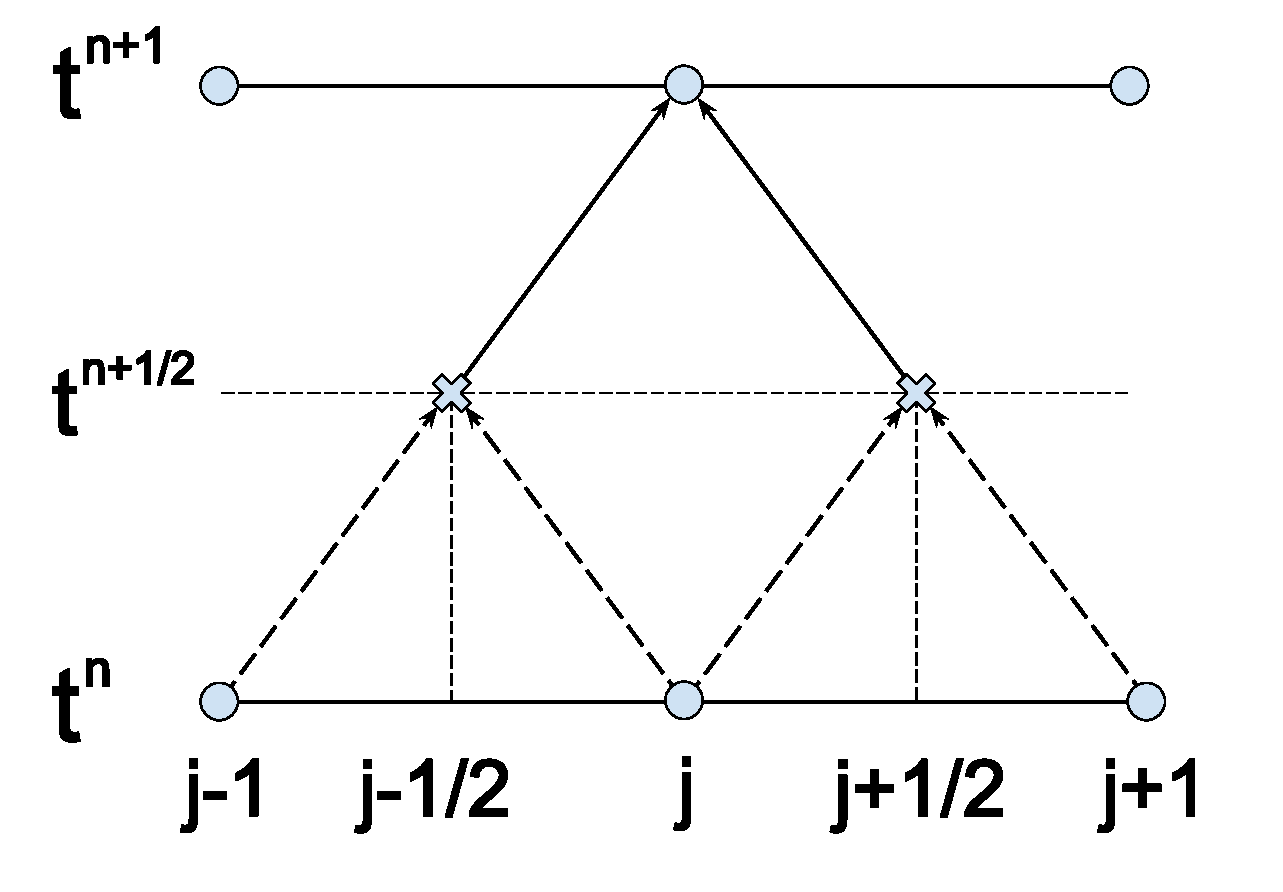
\includegraphics[width=0.8\textwidth]{Lax-Wendroff.pdf}
		\caption{Консервативный двухшаговый метод Лакса-Вендроффа на пространственно - временной сетке.}
		\label{LW_picture}
	\end{figure}
	Сетка для вычислений вводится следующим образом. Длина рассматриваемой области $l$ делится на выбранное количество узлов ячеек $N$ в итоге получаем сетку с узлами $j$ - 
	\[
		0 \leqslant j \leqslant N .
	\]
	Узлы с номерами 0 и N считаются граничными. Значения в этих узлах определяются начальными условиями и остаются постоянными на протяжении всего расчёта, либо устанавилваются наперёд заданной функцией, зависящей от времени.
	
	\section{Задача о линейном переносе}\label{transfer}
	Рассмотрим одно из уравнений вида \eqref{dudt}, являющееся законом сохранения массы в дифференциальнй форме - уравнение переноса:
	\begin{equation}
		\diffp{\rho}{t} + \nabla ( \rho \mathbf{v} ) = 0 .
	\end{equation}
	В одномерном случае $\mathbf{u} = \rho$ и $\mathbf{F} = \rho v$. Разностная схема соответствует приведённым в разделе \ref{Lax-Wendroff} уравнениям \eqref{LW_helper} -- \eqref{LW_main}.
	
	Начальные условия:
	\begin{equation}
		\begin{cases}
			\left.\mathbf{u}\right|_{t_0} = 0.8\:;		&		0.4 \leqslant x \leqslant 0.8 \, ,	\\
			\left.\mathbf{u}\right|_{t_0} = 0.4\:;		&		x < 0.4\,; x > 0.8 \, .
		\end{cases}
	\end{equation}
	\[
		\begin{aligned}
			x \in [0, 1] \\
			t \in [0, T]
		\end{aligned}
	\]
	Аналитическим решением уравнения адвекции является функция:
	\begin{equation}
		\mathbf{u}(t) = \mathbf{u}(0) + vt \: ,
	\end{equation}
	где $v$ - скорость распространения возмущения.
	
	
	
	\section{Основные уравнения}
	%Potter p.272
	Уравнения идеальной гидродинамики в дифференциальной форме относительно неподвижной системы отсчёта:
	\begin{gather}
		\diffp{\rho}{t} + \nabla ( \rho \mathbf{v} ) = 0 ,	\\[10pt]
		\diffp{\rho \mathbf{v}}{t} + (\nabla \rho \mathbf{v}) \mathbf{v} = -\nabla p ,	\\[10pt]
		\diffp{}{t}\left(\rho \varepsilon + \frac{1}{2} \rho v^2 \right) + 
						\nabla \left\{ \left( \frac{1}{2} \rho v^2 + \rho \varepsilon + p \right)\mathbf{v}\right\} = 0 ,
	\end{gather}
	где $\varepsilon$ -- удельная внутренняя энергия. Для иделального газа она выражается как:
	\begin{equation}
		\varepsilon = \dfrac{kT}{m(\gamma-1)} = \dfrac{p}{\rho (\gamma - 1)} ,
	\end{equation}
	где $\gamma$ -- показатель адиабаты (отношение теплоемкостей), $m$ -- масса молекулы (либо атома), $k$ -- постоянная Больцмана, $T$ - температура. 

	\section{Задача о гидродинамическом разрыве}\label{hydrodynamics}
	%Potter p.319
	Уравнения гидродинамики можно записать в консервативной форме следующим образом:
	
	где векторы физических величин и потоков равны, соответственно:
	\begin{equation}
	\mathbf{u}	=	\begin{vmatrix}
						\rho								\\
						\rho v								\\
						\frac{1}{2}\rho v^2 + \rho \varepsilon		
					\end{vmatrix} , \qquad	
	\mathbf{F}	=	\begin{vmatrix}
						\rho v								\\
						\rho v^2 + p								\\
						\left(\rho \varepsilon + \frac{1}{2}\rho v^2 + p\right)v	
	\end{vmatrix}	.		
	\end{equation}
	
	
\end{document}